\input{coconut-theme.tex}

\title{傑利蠑螈}
\subtitle{說明簡報}

\usepackage{graphicx}
\graphicspath{ {./images/} }

\begin{document}

% title
{\setbeamertemplate{footline}{}
\begin{frame}[plain]
  \centering
  \vspace{0.5cm}
  {\Huge\bfseries\textcolor{deepsea}{傑利蠑螈}}\\[0.2cm]
  {\LARGE\textcolor{ocean}{說明簡報}}\\[0.5cm]
  \begin{tikzpicture}
    \fill[ocean!25] (-5,-0.6) rectangle (5,0.1);
    \fill[sand] (0,0.05) ellipse (1.7 and 0.45);
    \begin{scope}[shift={(0,0.05)}]\upsidedowntree\end{scope}
  \end{tikzpicture}\\[0.3cm]
  {\large\textcolor{coconut}{2026 資訊營・賽局・關卡三}}
\end{frame}}

% preface
\begin{frame}{劇情}
  \vspace{0.8em}
  \begin{oceanbox}
    \large
    一群人被丟到了荒涼的海島上，而你（一個小隊）是其中之一。為了要爭奪誰是老大，你們按地裡各懷鬼胎，希望能得到最多人的擁戴。好在你從海盜那裡學會了專屬南洋的魔法，除了能夠洗腦島上的動物支持你之外，還能胡亂分配選區以最大化支持度，你能夠成為島嶼的霸主嗎...抑或是成為他人的奴隸呢...
  \end{oceanbox}
  \vspace{1em}
  \begin{center}
  \begin{tikzpicture}[scale=1.1]
    \fill[sun!70] (-3.4,1.6) circle (0.35);
    \fill[ocean!25] (-4.2,-0.7) rectangle (4.2,-0.1);
    % 椰子島
    \fill[sand] (2.4,-0.15) ellipse (1.5 and 0.4);
    \begin{scope}[shift={(2.4,-0.05)}]\upsidedowntree\end{scope}
    % 獨木舟
    \draw[line width=3pt, coconut] (-2.6,-0.45) .. controls (-1.8,0.05) and (-1.0,0.05) .. (-0.2,-0.45) -- cycle;
    \fill[coconut!80] (-2.5,-0.45) .. controls (-1.8,-0.05) and (-1.0,-0.05) .. (-0.3,-0.45) -- cycle;
  \end{tikzpicture}
  \end{center}
\end{frame}

% page 
\begin{frame}{遊戲目標與大綱}
  \vspace{0.4em}
  % \large
  分配支持者、劃定選區，最終獲取最多的支持者！
  \begin{figure}[hcp]
    \centering
    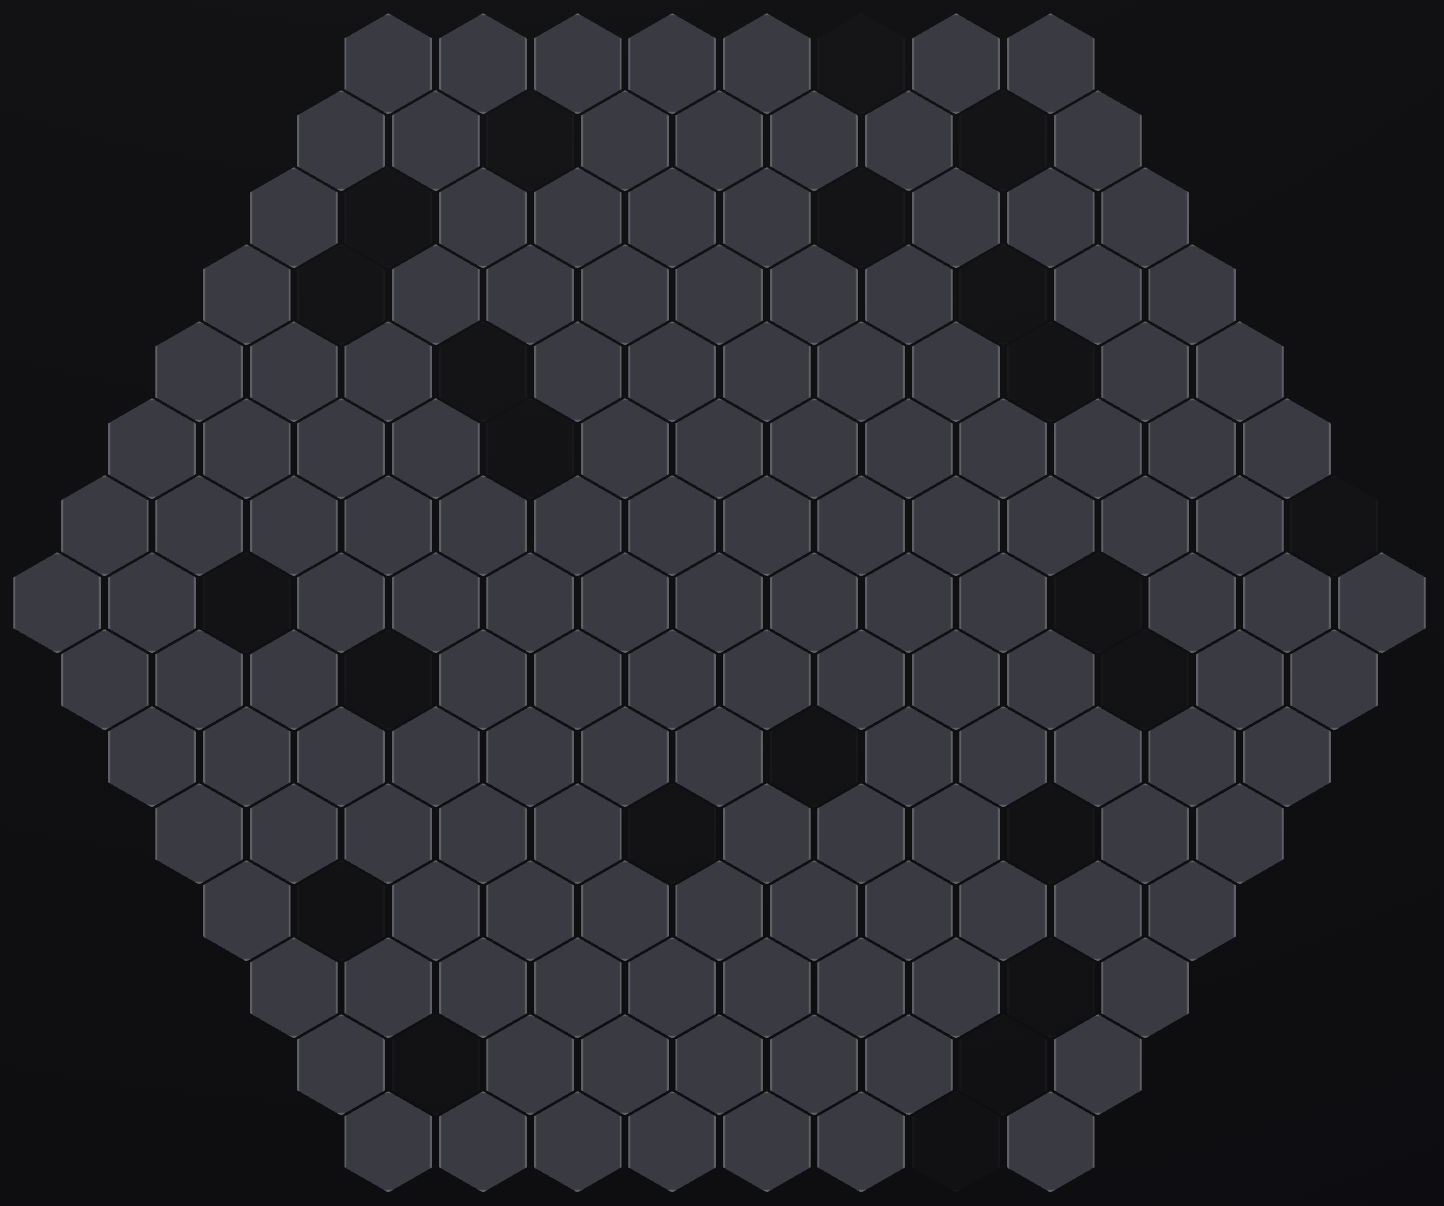
\includegraphics[width=0.32\textwidth]{blank}
    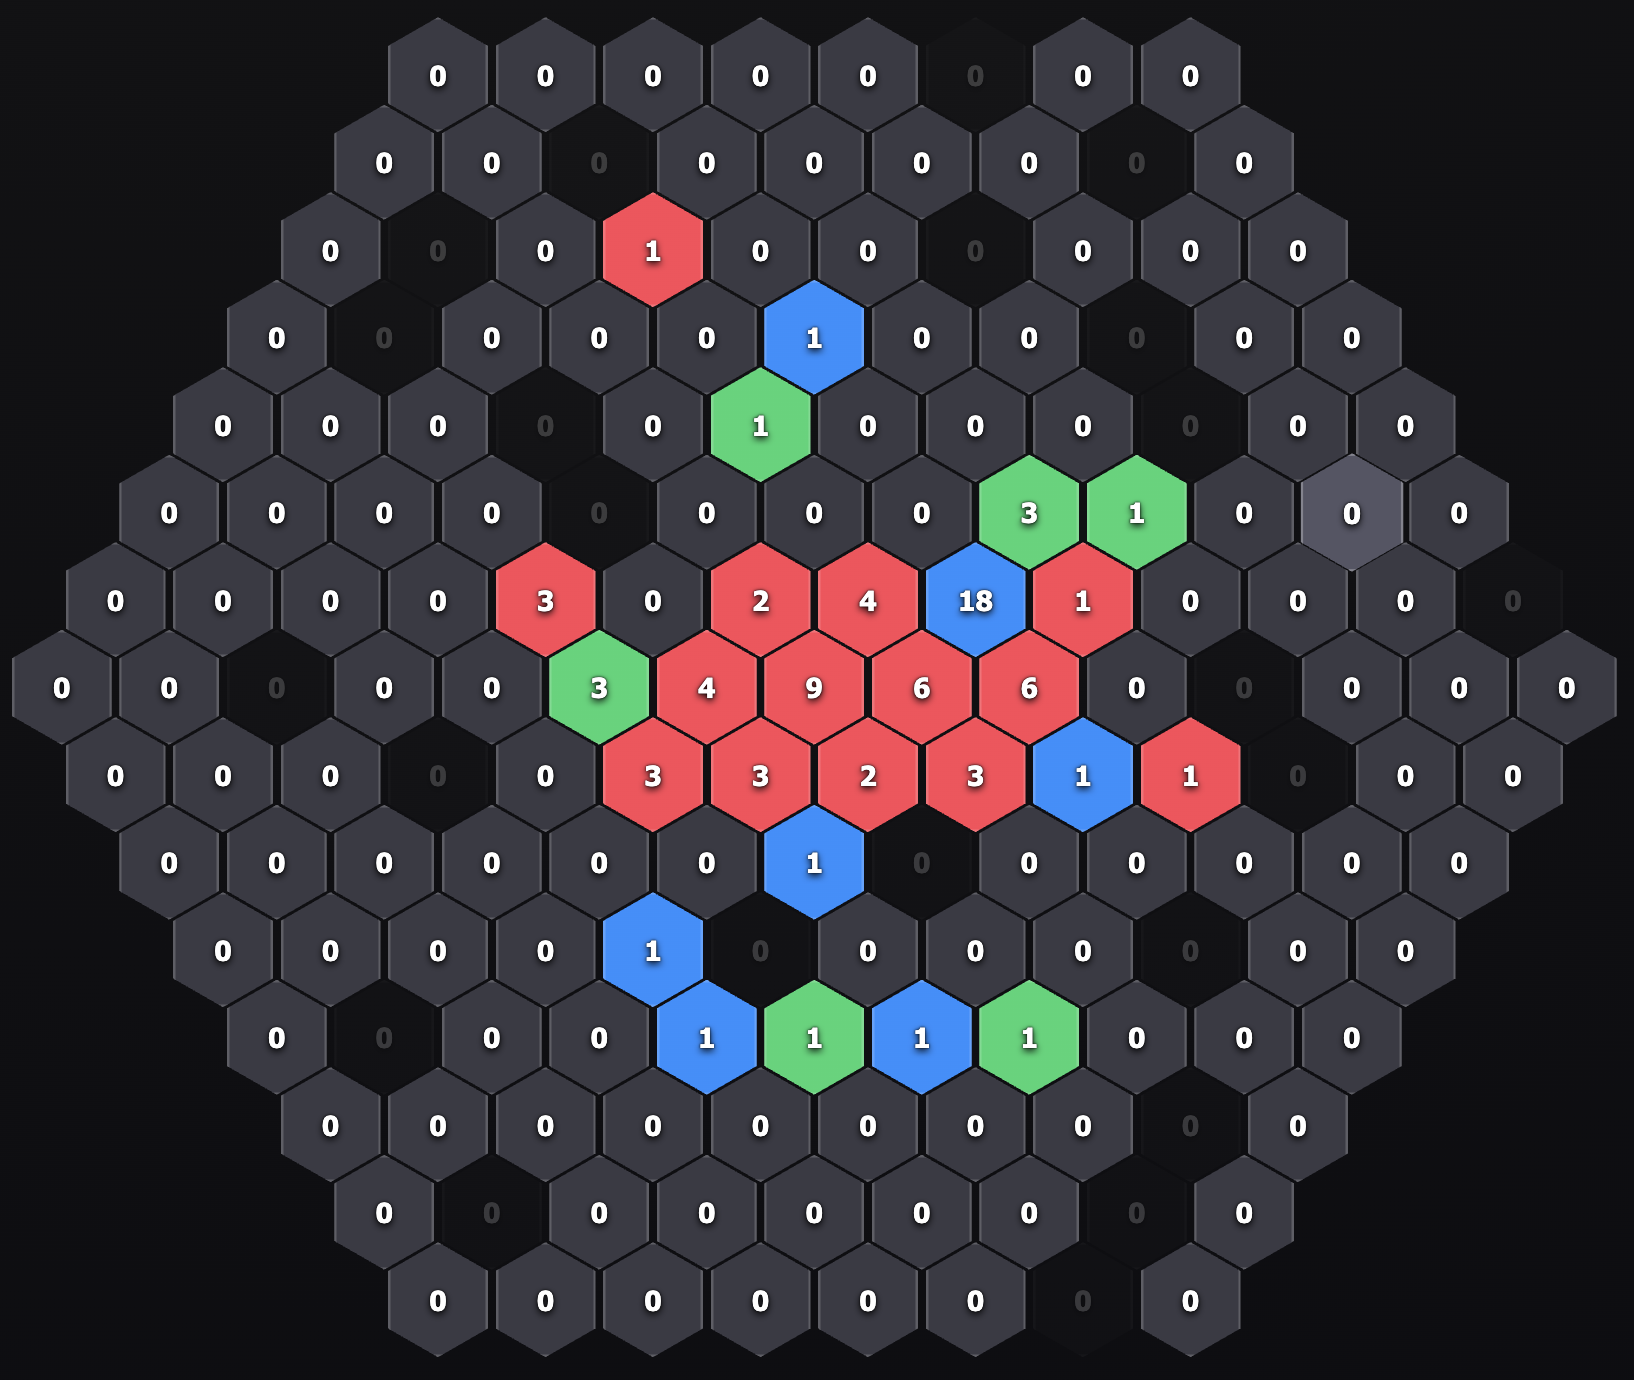
\includegraphics[width=0.32\textwidth]{some}
    \vfill
    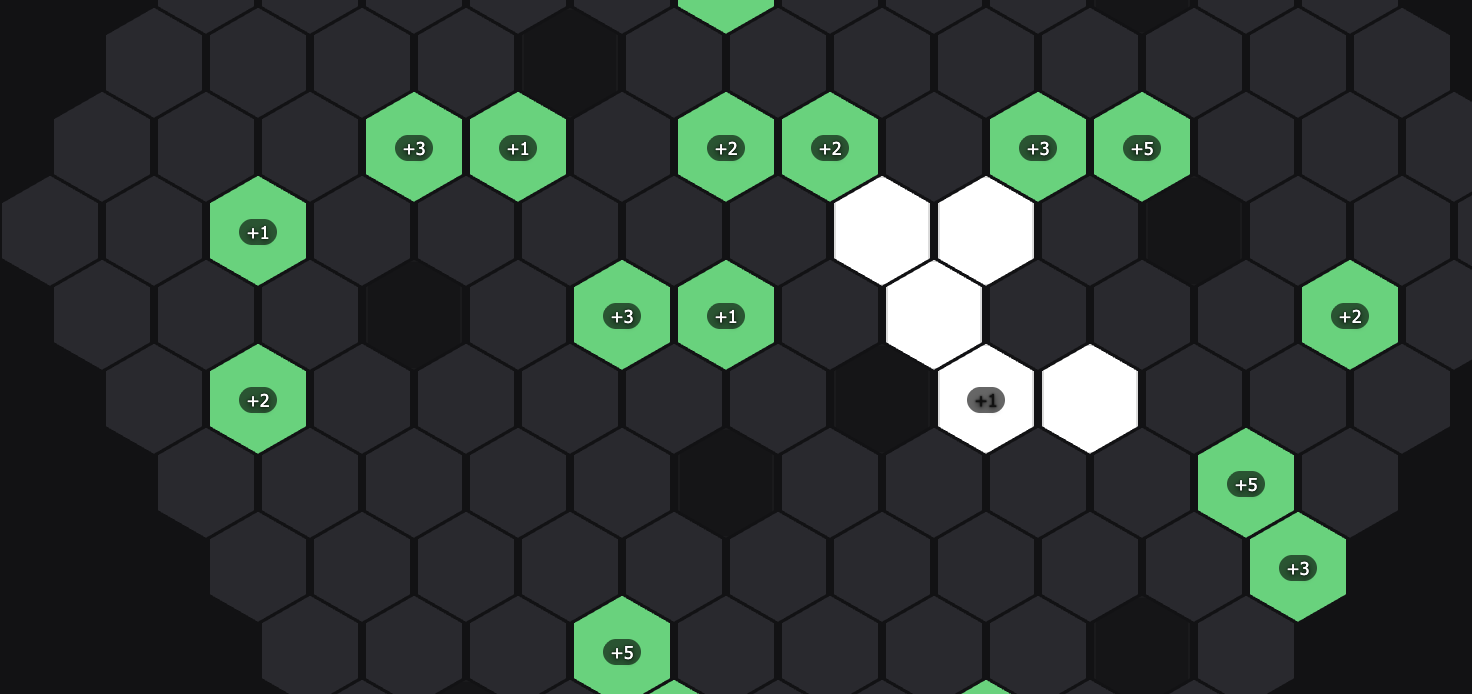
\includegraphics[width=0.32\textwidth]{placement}
    \vfill
  \end{figure}
\end{frame}

% page 
\begin{frame}{島嶼與棲地} 
  \vspace{0.4em}
  \large
    一個六角形的網格為一塊\textbf{棲地}，許多棲地共同組成\textbf{島嶼}。
\vspace{0.4em}

\centering
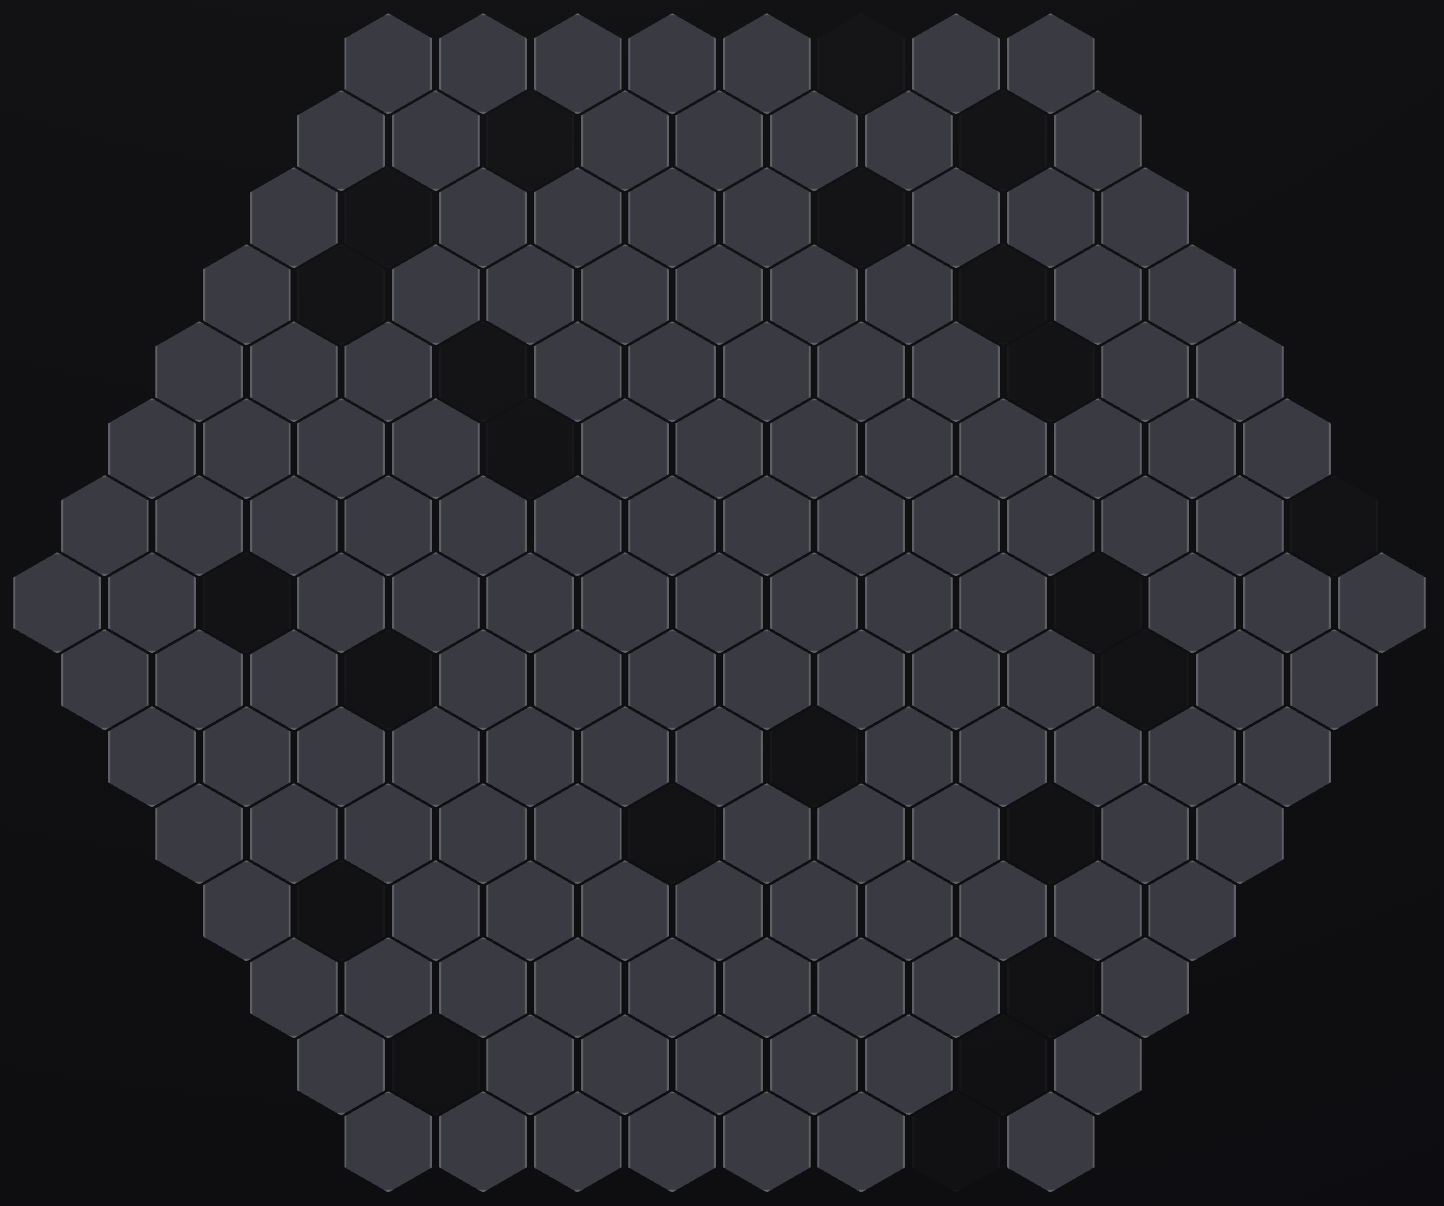
\includegraphics[width=0.5\textwidth]{blank}
\end{frame}

% page 
\begin{frame}{猴子}
  \vspace{0.4em}
    \large
    每隻\text{猴子}代表支持某小隊的勢力，可以把猴子分配到棲地上。

\vspace{0.4em}

\centering
% 
\includegraphics[width=0.32\textwidth]{ballots}
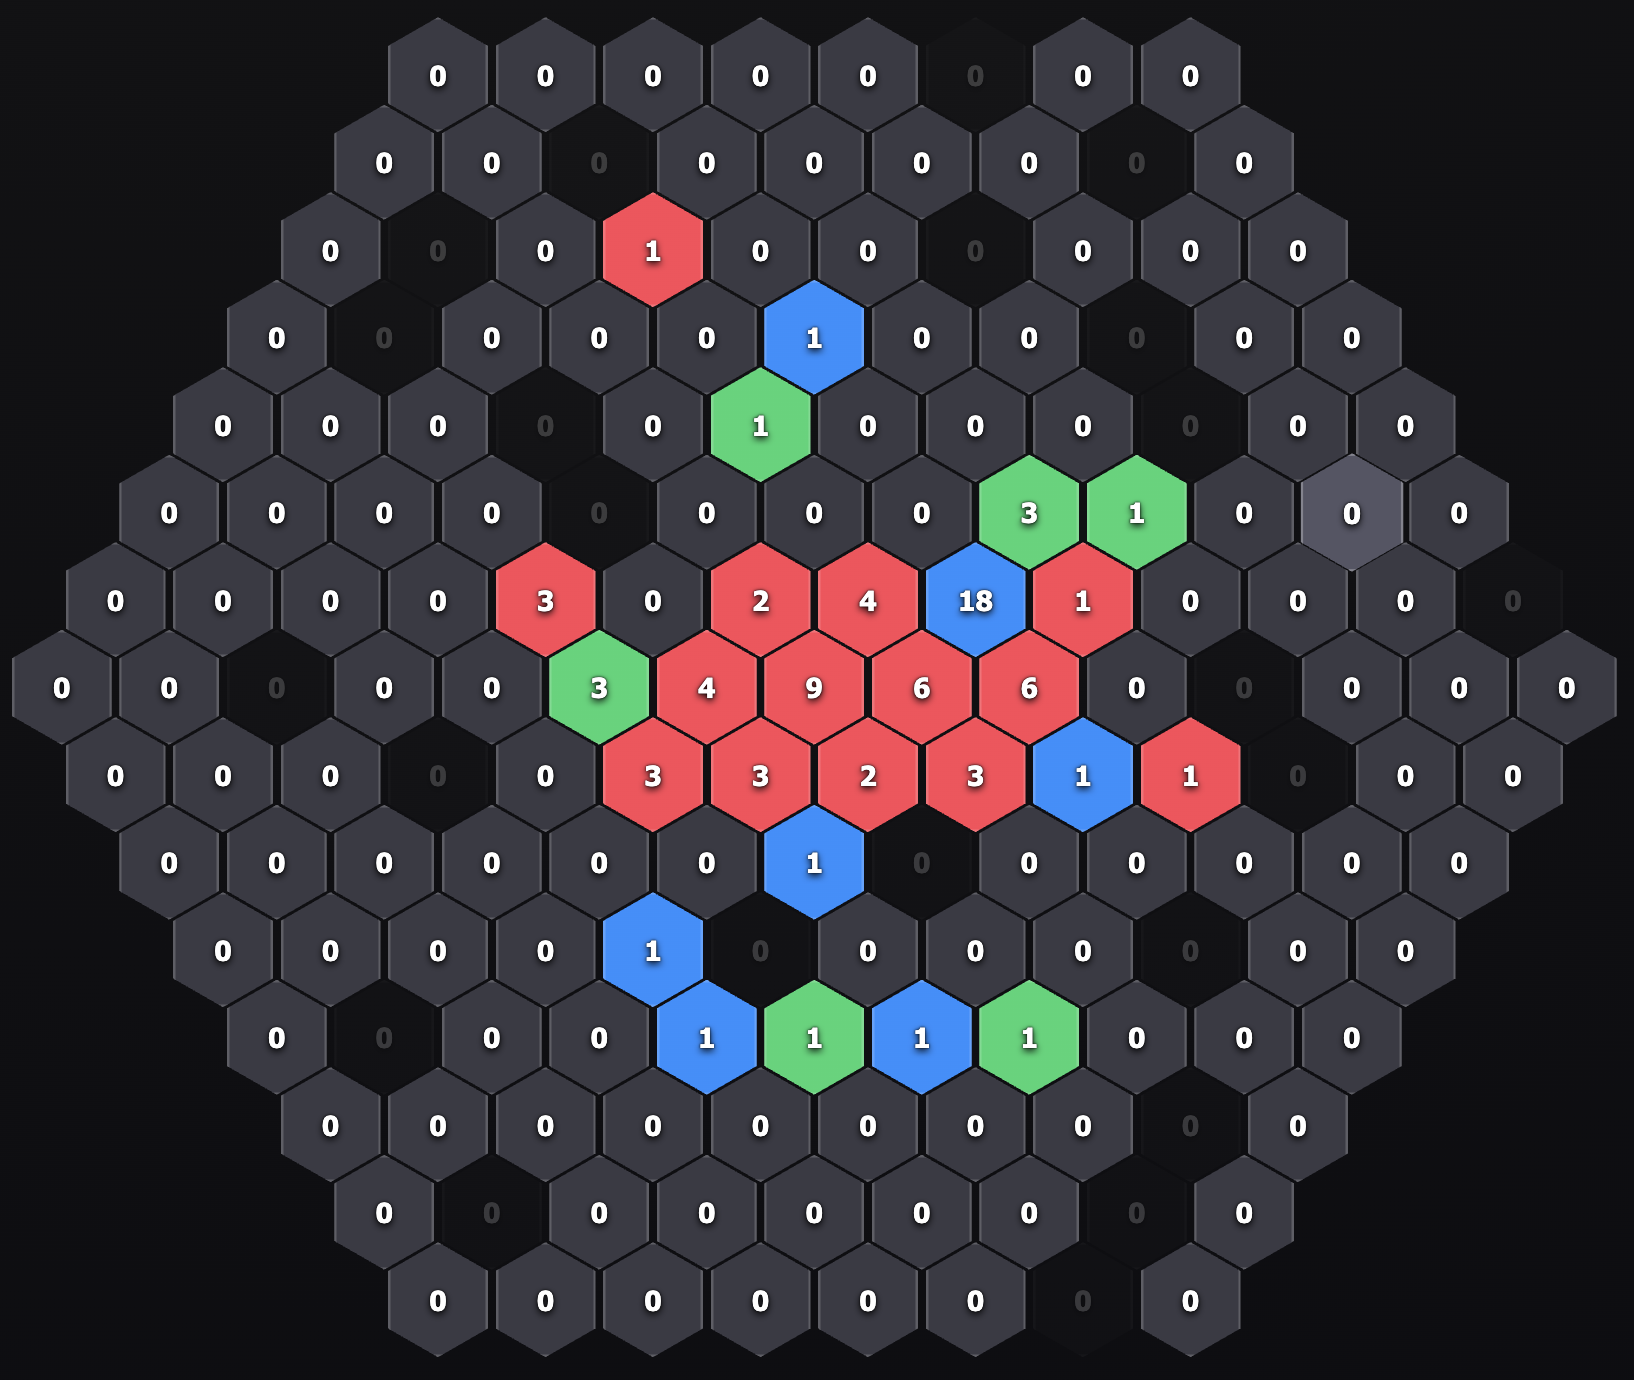
\includegraphics[width=0.5\textwidth]{some}
\end{frame}

% page 
\begin{frame}{遊戲流程}
  \vspace{0.4em}
  \large
  遊戲共有兩個階段，第一階段小隊要在島嶼的各個棲地上分配自己的支持者，第二階段則是將多個棲地用板塊劃到一起，試圖讓板塊中多數的猴子都支持自己。
\end{frame}

% page 
\begin{frame}{階段一：分配勢力}
  \vspace{0.4em}
  \begin{itemize}
    \item 共進行三輪，每輪 3 分鐘
    \item 每輪每隊最多可以分配 100 隻猴子
    \item 第一輪每格每隊最多放 20 隻猴子、第二輪 25 隻、第三輪 30 隻
    \item 前兩輪結束皆會公布所有小隊的分配情形
  \end{itemize}
\vspace{0.4em}

    \centering
    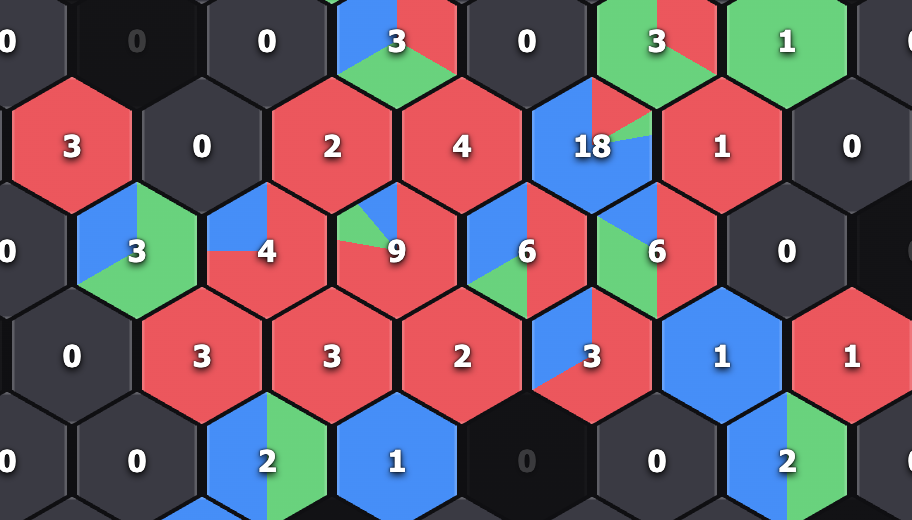
\includegraphics[width=0.6\textwidth]{anno}
\end{frame}

% page 
\begin{frame}{搶奪他人的猴子！}
  \vspace{0.4em}
    同一棲地內的猴子會轉而支持原先在該棲地內獲得多數支持的小隊
  \begin{itemize}
    \item 三輪結束後將進行猴子內戰
    \item 每個棲地內有最多數量猴子的小隊將可以獲得該棲地內所有猴子
    \item 若不存在絕對多數，則棲地內所有猴子都會集體消失
  \end{itemize}
\vspace{0.4em}

    \centering
    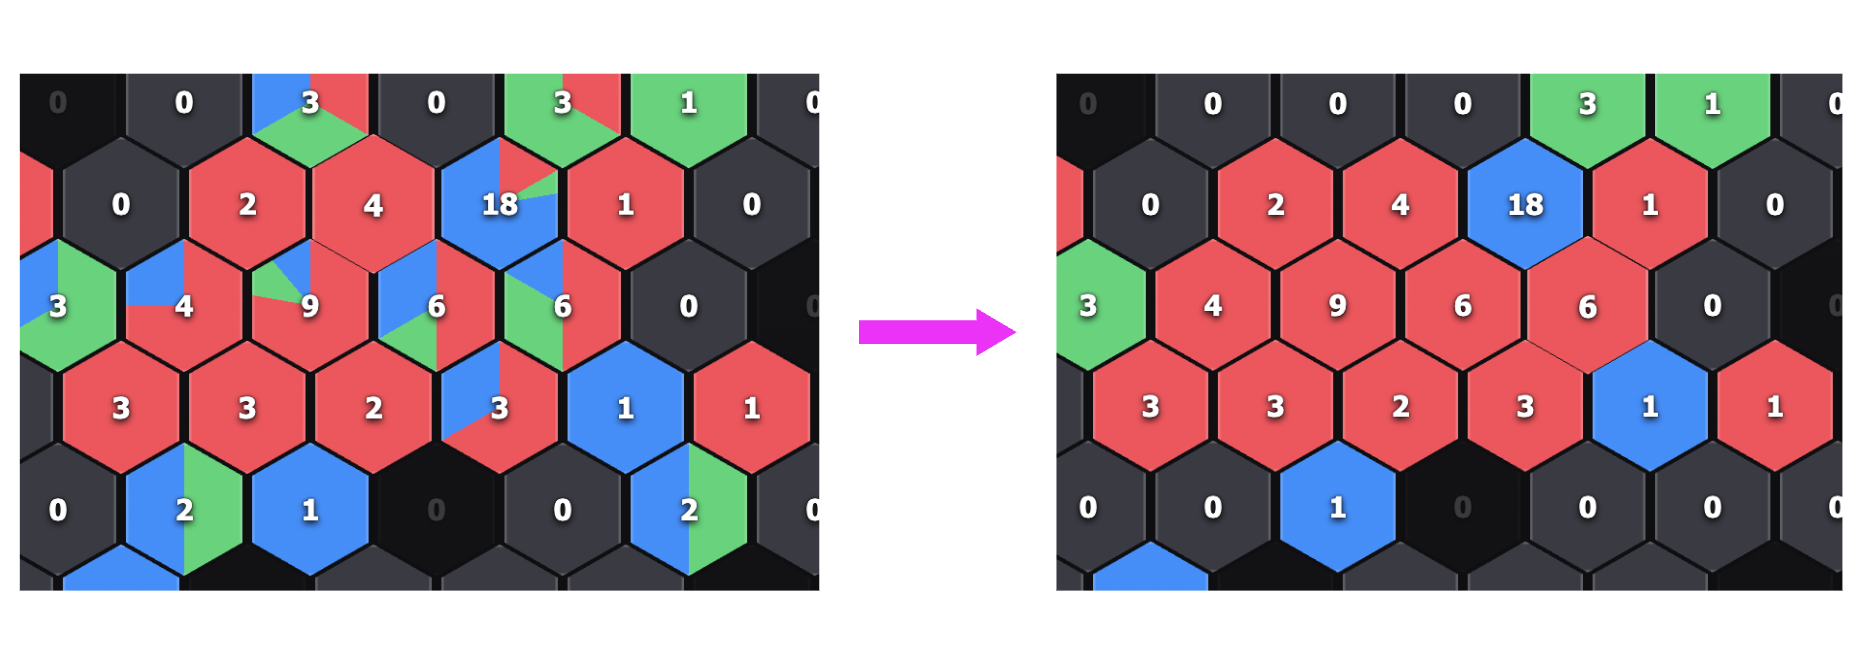
\includegraphics[width=0.6\textwidth]{distri}
\end{frame}

% page 
\begin{frame}{階段二：傑利蠑螈}
  \vspace{0.4em}
  \begin{itemize}
    \item 每個小隊有一些包含五個相連棲地的板塊，階段ㄧ即可預覽
    \item 小隊依\textbf{階段一}放置猴子的變異數由大至小輪流放板塊
    \begin{itemize}
      \item 只考慮有放的格子
    \end{itemize}
    \item 放置時限 30 秒
  \end{itemize}
  \vspace{0.4em}

    \centering
    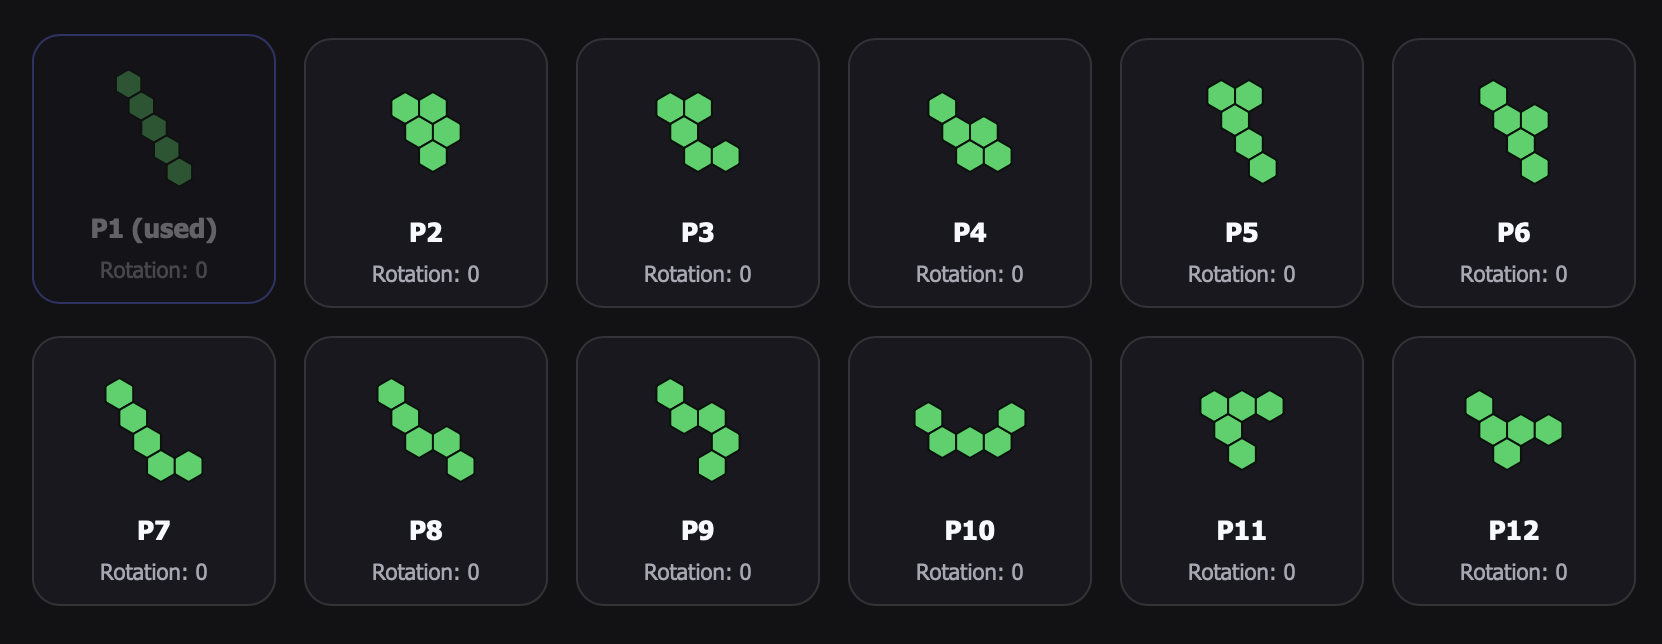
\includegraphics[width=0.55\textwidth]{clusters}
\end{frame}

% page 
\begin{frame}{俗話說得蠑螈者得天下}
  \vspace{0.4em}
  \begin{itemize}
    \item 五格內有最多猴子支持的小隊獨得所有猴子
    \item 點兩下可以旋轉板塊、拖曳可以放置
    \item 注意時間！！！
  \end{itemize}

  \vspace{0.4em}

    \centering
    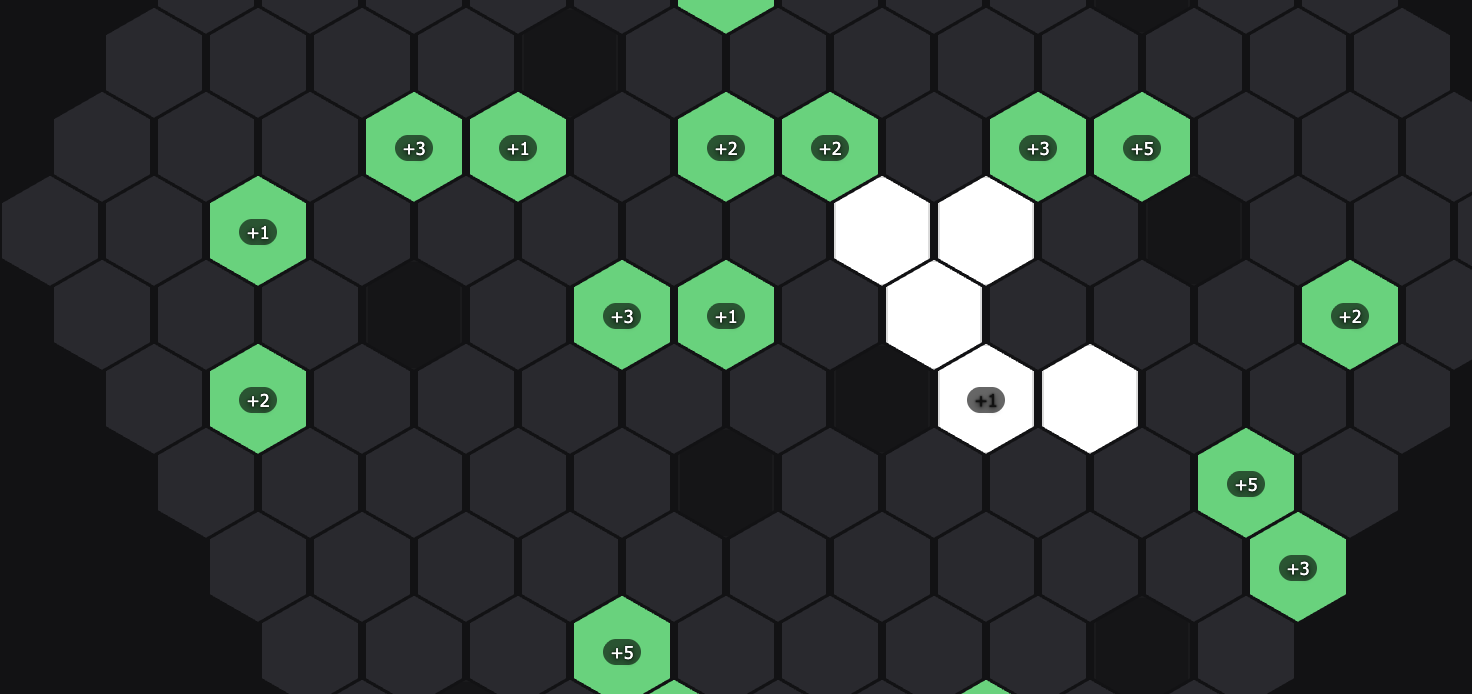
\includegraphics[width=0.55\textwidth]{placement}
\end{frame}

% page 
\begin{frame}{成績結算}
  \vspace{0.4em}
  \begin{itemize}
    \item 依照獲得的票數，第一名至第十名分別獲得以下分數
  \end{itemize}

    \begin{table}[hc]
\centering
\begin{tabular}{|c|c|}
\hline
    \textbf{名次} & \textbf{分數} \\ \hline
    ㄧ & 10 \\ \hline
    二 & 9 \\ \hline
    三 & 8 \\ \hline
    四 & 7 \\ \hline
    五 & 6 \\ \hline
    六 & 5 \\ \hline
    七 & 4 \\ \hline
    八 & 3 \\ \hline
    九 & 2 \\ \hline
    十 & 1 \\ \hline
\end{tabular}
\label{tab:example}
\end{table}
\end{frame}

% page 
\begin{frame}{LINK}
  \vspace{0.4em}
  \centering

\begin{itemize}
  \item \texttt{https://csiecamp.csie.org/gerrymandering}
    \item 帳密：\texttt{group\#}
    \item 請每隊使用\textbf{一台電腦}登入
\end{itemize}
  
\end{frame}

\end{document}
